%%%%%%%%%%%%%%%%%%%%%%%%%%%%%%%%%%%%%%%%%
% Stylish Article
% LaTeX Template
% Version 2.1 (1/10/15)
%
% This template has been downloaded from:
% http://www.LaTeXTemplates.com
%
% Original author:
% Mathias Legrand (legrand.mathias@gmail.com) 
% With extensive modifications by:
% Vel (vel@latextemplates.com)
%
% License:
% CC BY-NC-SA 3.0 (http://creativecommons.org/licenses/by-nc-sa/3.0/)
%1
%%%%%%%%%%%%%%%%%%%%%%%%%%%%%%%%%%%%%%%%%

%--------------------------------------------------------------# Path to your oh-my-zsh installation.--------------------------
%	PACKAGES AND OTHER DOCUMENT CONFIGURATIONS
%----------------------------------------------------------------------------------------

\documentclass[fleqn,10pt]{SelfArx} % Document font size and equations flushed left

\usepackage[english]{babel} % Specify a different language here - english by default

\usepackage{marvosym, epigraph, subfig}

\usepackage[sortcites=false,style=authoryear-comp,bibencoding=utf8, natbib=true, firstinits=true, maxcitenames=2, maxbibnames = 99, uniquename=false, backend=bibtex, useprefix=true, backref=false,doi=false,isbn=false,url=false,dashed=true]{biblatex}
\setlength\bibhang{20pt}
\bibliography{ThomasReferenties.bib}
\AtEveryBibitem{%
	\clearfield{day}%
	\clearfield{month}%
	\clearfield{endday}%
	\clearfield{endmonth}%
}

%----------------------------------------------------------------------------------------
%	COLUMNS
%----------------------------------------------------------------------------------------

\setlength{\columnsep}{0.55cm} % Distance between the two columns of text
\setlength{\fboxrule}{0.75pt} % Width of the border around the abstract

%----------------------------------------------------------------------------------------
%	COLORS
%----------------------------------------------------------------------------------------

\definecolor{color1}{RGB}{0,0,90} % Color of the article title and sections
\definecolor{color2}{RGB}{0,20,20} % Color of the boxes behind the abstract and headings

%----------------------------------------------------------------------------------------
%	HYPERLINKS
%----------------------------------------------------------------------------------------

\usepackage{hyperref} % Required for hyperlinks
\hypersetup{hidelinks,colorlinks,breaklinks=true,urlcolor=color2,citecolor=color1,linkcolor=color1,bookmarksopen=false,pdftitle={What drives which region?},pdfauthor={Thomas de Graaff}}

%----------------------------------------------------------------------------------------
%	ARTICLE INFORMATION
%----------------------------------------------------------------------------------------

\JournalInfo{Research agenda, 2017--2021} % Journal information 
\Archive{Position paper} % Additional notes (e.g. copyright, DOI, review/research article)

\PaperTitle{Do regional economists answer the right questions?}
\SubPaperTitle{On the current discrepancy between the questions regional economists solve and the questions policy makers actually ask}

\Authors{Thomas de Graaff\textsuperscript{1}*} % Authors
\affiliation{\textsuperscript{1}\textit{Department of Spatial Economics, Vrije Universiteit Amsterdam, Amsterdam, The Netherlands}} % Author affiliation
\affiliation{*\textbf{Corresponding author}: \Letter{} t.de.graaff@vu.n; \Mundus{} \href{thomasdegraaff.nl}{thomasdegraaff.nl}} % Corresponding author

\Keywords{Regional economics --- predicting --- causality --- theory driven
  approach --- data science}
\newcommand{\keywordname}{Keywords} 

%%----------------------------------------------------------------------------------------
%%	ABSTRACT
%%----------------------------------------------------------------------------------------

\Abstract{This position paper revolves around two main propositions: namely,
  (\textit{i}) regional (or spatial) economists are very restrictive in the tool
  set they apply, and consequently (\textit{ii}) their models do not always
match with the type of questions policy makers are concerned about. To start
with the latter, policy makers---whether national, regional or local---are
oftentimes concerned about holistic approaches and future predictions. Exemplary
questions are ``Which policy instrument works best for my city'', ``What
happens after the construction of this highway with housing prices and
employment throughout the whole region'' and ``Given limited budget, which
region should I first invest in''. Regional economists---actually, most economists---usually isolate phenomena in order to, at best, explain the impact of a single determinant. Indeed, most regional economists feel very uncomfortable when asked to predict or give the best set of determinants for a certain phenomenon. This has its consequences for the tool set regional economists apply. Usually a parametric regression type of framework is applied isolating the determinant under consideration and controlling as much as possible for observables and unobservables, ideally in a pseudo-experimental framework. A direct consequence of this approach is that emphasis is very much on explaining the impact of an isolated determinant and not on predicting (non-marginal) changes in larger systems. For many applications that is definitely the right approach. However, as this paper ultimately argues, it is very much as well a selective approach that does not do well to deliver on some of the questions policy makers ask regional economists.}

%----------------------------------------------------------------------------------------

\begin{document}

\flushbottom % Makes all text pages the same height
\maketitle % Print the title and abstract box
%\tableofcontents % Print the contents section
\thispagestyle{empty} % Removes page numbering from the first page

%----------------------------------------------------------------------------------------

\section*{Introduction: two different cultures} % The \section*{} command stops section numbering

\addcontentsline{toc}{section}{Introduction: two different cultures}

\epigraph{The sexiest job in the next 10 years will be statisticians.}{Hal Varian, 2009}

The quote above from Hal Varian is in one aspect wrong; nowadays, we do not call
them statisticians but data scientists instead. Nevertheless, in the last two
decades companies such as Google, Ebay, Whatsapp, Facebook, Booking.com and
Airbnb, have not only witnessed enormous growth but to a considerable extent also changed the socio-economic landscape. Indeed, with the increasing abundance of (spatial) data and computer capacity, the ability to gather, process, and visualize data has become highly important and therefore highly in demand as well. And all the models and tools these data scientists within these companies use are very much \textit{data driven} with often remarkable results. 

In his controversial and path-breaking article, \citet{breiman2001statistical}
presented two different cultures in statistical science. One governed by
a (probability) theory-driven modeling approach and one governed by a more (algorithmic) data-driven approach. These two cultures carry over to the econometric and ultimately the
empirical regional economics domain\footnote{I use a wide definition for the regional economics
 domain, which consists of most aspects of regional science in general but for
 which the theoretical approach is always from an economic perspective. Topics
 such as, e.g, interregional migration, trade, transport flows and commuting on
 the one side and regional performance, regional clustering, population growth and
 specialisation on the other side fall all under this, admittedly, rather wide umbrella.} as well, where---commonly for all social
sciences---the theory driven approach still very much dominates the landscape of the realm of contemporary regional economics. 

\begin{figure*}[t!]\centering 
	\subfloat[Theory or modeling approach\label{modelapproach}]{%
		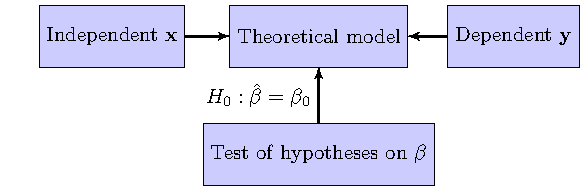
\includegraphics[width=0.49\textwidth]{./figures/modelapproach}
	}
	\hfill
	\subfloat[Data driven approach\label{dataapproach}]{%
		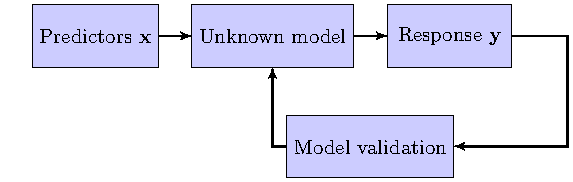
\includegraphics[width=0.49\textwidth]{./figures/dataapproach}
	}
0	
	\caption{Two cultures of statistical/econometric modeling \citep[inspired by][]{breiman2001statistical}}
	\label{fig:twocultures}
\end{figure*}

Figure \ref{fig:twocultures} is an adaptation from the one displayed in \citet{breiman2001statistical} and describes the processes governing these two cultures. Figure (\ref{modelapproach}) is what I refer to as the modeling approach, where a statistical model is postulated and is central to this culture. This is the classical approach\footnote{Sometimes as well referred to as the frequentists' approach. However, this typically concerns the debate between classical statistics and Bayesian statistics, where the two approaches I refer to are more concerned with wider frameworks, of which the Bayesian approach is just one of the elements.} where statistical probability theory meets the empiricism of Karl Popper. Usually the model assumed is stated as a linear model and in its most simple form can be denoted as:
\begin{equation}
	\mathbf{y} = \mathbf{x}\beta + \epsilon, 
\end{equation}
where in (regional) economics language, $\mathbf{x}$ is referred to as the
independent variable, $\mathbf{y}$ as the dependent variable and $\epsilon$ as a
residual term. In this setup, using the data at hand, one constructs a
statistical test to which extent the estimated coefficient (denoted with
$\hat{\beta}$) deviates from a hypothesized value of the coefficient (denoted
with $\beta_0$)---typically the hypothesis $H_0: \hat{\beta} = 0$ is used with
as alternative hypothesis that $H_1: \hat{\beta} \neq 0$. However, that is
always within the context of the \textit{postulated} model. So, when the
null-hypothesis is rejected, it not necessarily means that the true $\beta$ is
unequal to zero, it might also be caused by errors in measuring $\bf{x}$ or even
using the wrong \textit{model}!\footnote{One of the assumptions for regression
  techniques such as the one used here is actually no misspecification of the
  model, but---apart from some possible tests on the functional form
  \textit{within} a specific regression form---usually little attention is give
  on the validity of the model used. More importantly, within this framework the
  model itself is usually not tested \textit{a posteriori}.}\footnote{There is
  another fallacy with this approach that is often overlooked and that is that
  the alternative hypothesis being true is a probability as well. Namely,
most hypotheses researchers test are typically not very probable. Not taken this
into account would actually lead to more null hypotheses to be rejected then
should be (false positives).}

Therefore it is striking that in economics in general, and in regional economics
in specific, most of the tools employed are very much \textit{theory or model
  driven} instead of data driven. My (conservative) estimate would be that 90\%
of all empirical work in regional economics revolves around postulating a
(linear) model and testing whether (a) key determinant(s) are significantly
different from a hypothesized value---usually zero.\footnote{In a seminal
  contribution, \cite{breiman2001statistical} states that deep into the 90s 98\%
  of the statisticians actually employed the theory driven paradigm and only 2\%
  a data driven paradigm. With the advent of the availability of internet
  connectivity, large (online) data sources, and faster computers the
  statistical realm changed dramatically. However, this has not permeated yet in
  the social sciences \citep[see as well][]{varian2014big}} That is, \textit{within} the context of the model assumed.

At best, this approach can be seen in a causal inference framework. If a
determinant (such as a policy in the context of economics) $x$ changes, does it
cause then a change in the output $y$ (most economists typically use some welfare measure).\footnote{Most of this research actually intends to mimic a \textit{difference-in-difference} approach and gained enormous momentum with the textbook of \citet{angrist2008mostly}.} This approach thus provides a rigid and useful approach to regional policy evaluation. If we implement policy $x$, does welfare measure $y$ then improve? 

However, policy makers oftentimes have different questions for which they need
solutions. Usually, they revolve around questions starting with \textit{``What
  determines performance measure $A$?''}, \textit{``Which regions can we best
    invest in?''} or, more generally, \textit{``What
  works for my region?''}. These types of questions require a different approach
than the previous one. Namely, the former type requires an approach focused on \textbf{explaining} while the latter type requires an approach focused on \textbf{predicting}.

Figure (\ref{dataapproach}) yields a schematic overview of a more data driven
approach. Here, we see an unknown model fed by predictors $\mathbf{x}$ that lead
to one or multiple reponses $\mathbf{y}$. The main objective here is not to test
hypotheses, but to find the best model instead able to explain the data.
Usually, the models are evaluated by some kind of criterion (e.g., mean squared
error), which is not completely unlike the modeling approach. However, there are
two main differences between the two approaches. First, the data driven approach
considers several models in a structural approach. For instance, the question
which variables to include is captured by an exhaustive sourse of all
combinations in the modeling approach (e.g., with classification and regression
trees or random forests), while in the theory driven approach, the choice of
variables is based on the theory and a small number of variations in the
specification. Second, measurements on model performance are done
\textbf{out-of-sample} in the data driven approach and, typically,
\textbf{in-sample} in the model approach. The latter is not that important for
hypothesis testing, but for prediction this matters enormously, because adding
parameters might increase the in-sample fit, but actually worsen the
out-of-sample fit (overfitting).  


The remaining part of this position paper is structured as follows. Section
\ref{practices} gives an overview of current modeling practices and describes the `traditional'
inference based approach as well as some data-driven approaches that have been
used in the recent past (though by far not as often as the traditional methods).
Section \ref{agenda} sets out both a research and an education agenda as it
addresses how to bridge the gap between the daily practices of regional
economists and the demands of local policy makers. The final section shortly
summarizes the main points raised in this position paper.  

%------------------------------------------------

\section{Regional economists turning the blind eye\label{practices}}

Unmistakenly, in the recent decade the two major changes to economic empirical research in general
are the advent of increasingly larger data sources and the large increase in
computer power \citep[]{einav2014economics}. The methods that mosts economists
employ, however, have not changed. Linear regression or one of its close
relatives (such as logistic, poisson or negative binomial regression), preferably in a causal
framework, is still the most common tool. This also applies to regional
economists, who---although coming from a tradition to use various methods from
different disciplines---have increasingly used similar methods as in
``mainstream'' economics.

This focus on marginal effects and causality is
certainly very worthwhile and brought us many important insights. However, it is
also typically done within a very narrow framework and, below, I will lay out what we are missing both in
research and in our educational curricula, when our \emph{main} focus is on the
framework above and as advocated so much as in \citet{angrist2008mostly}.   

\subsection{The blind eye in research}

The traditional model of a (regional) economist looks as follows:
\begin{equation}
  \label{model_economist}
  y_i = \alpha + \beta x_i + \mathbf{z}_i\gamma + \epsilon_i,
\end{equation}
where $y_i$ is referred to as the dependent variable, $x_i$ is the main variable of
interest, and $\mathbf{z}$ is a vector of other variables. $\alpha$, $\beta$ and
$\gamma$ are parameters, where we are especially interested in the value of
$\beta$. Finally, $\epsilon_i$ is an identical and independent distributed error
term.

The main aim is to estimate $\beta$ as unbiased as possible. So, ideally, we
would like to control for unobserved heterogeneity bias, specification bias,
measurement error, reverse causality, selection bias, and so forth. Econometric
theory has produced some very powerful techniques to control for some of these
biases, such as instrumental variables, diff-in-diff procedures and the use of
fixed effects. However, these methods are not panacea for everything. First, they work
wonders for only specific research questions that have to do with the marginal effects of
marginal changes. Second, some of these techniques require very specific and
strong assumptions which are possibly not always met, which leaves doubts upon
the validity of the results 

Below, I will deal with instrumental variables, diff-in-diff and fixed effect
techniques. I will specificially focus on some of the disadvantages. Some of the
arguments are adaptions from \citet{deaton2010instruments} and I refer to this
reference for a more complete treatise on the disadvantages of using
instrumental variables and diff-in-diff methods. For all the advantages,
read \citet{angrist2008mostly}. 

\subsubsection{Exogeneity versus independence}

Economists love instrumental variables, because a good instrumental variable can
tackle reverse causality, measurement error and unobserved heterogeneity bias
all at one. Originally, instrumental variables come from simultaneous economic
models such as supply and demand models. A classical example in a regional
context would be:
\begin{align}
  P_r &=  \alpha + \beta E_r + \mathbf{z}_r\gamma + \epsilon_r, \label{P}\\
  E_r &=  \delta + \kappa P_r+ \mathbf{w}_r\lambda + \nu_r,\label{E}
\end{align}
where $P$ denotes population, $E$ employment and $z$ and $w$ are vector of other
regional $r$ characteristics. $\alpha$, $\beta$, $\gamma$, $\delta$, $\kappa$
and $\lambda$ are parameters to be estimated.

Obviously, one can not directly estimate (\ref{P}) and (\ref{E}) because of the
intrinsic simultaneity. However suppose one is interested in estimating the
impact of employment on population growth, then one can use (\ref{E}) and seach
for \emph{exogeneous}\footnote{This is not really precise; I mean exogeneous to
  population variation. I will come back to the use of exogeneous later.} variation in employment to use it as an instrumental
variable. A possible strategy could be to look into the population changes of
surrounding regions (but within commuting distance), as they might not have an
impact of the population change in the current region
\citep[see][]{DeGraaff2012, Graaff2012}

The main point, however, is that equations (\ref{P})--(\ref{E}) constitute a full-blown
economic \emph{model} which has direct relations with the theoretical model of \citet{roback1982wages}. 

\subsubsection{Local average treatment effects}

\subsubsection{Fixed effects and heterogeneity}

\subsection{The blind eye in education}

%------------------------------------------------

\section{Incorporating the data science culture\label{agenda}}

What do we need?

\subsection{For research}

\subsubsection{Regional heterogeneity}

\citep{Thissen2016, Graaff2012, DeGraaff2012}

\subsubsection{Conditional robustness}

In regional science in general and in regional economics in specific, remarkably little attention has been given to reproducibility and robustness of results \citep[with some exceptions as, amongst some others, by][]{Rey:2014cl,arribas2015woow, Arribas2016}.

\subsubsection{Regional sorting models}

As in \citet{Bayer2004, Bayer2007a} and recently by \citet{Wang2016} and \citet{Bernasco2016}.

\subsection{For education}

\citet{schwabish2014economist}

\section{Into the abyss}

%----------------------------------------------------------------------------------------
%	REFERENCE LIST
%----------------------------------------------------------------------------------------

\addcontentsline{toc}{section}{References} % Adds this section to the table of contents
\printbibliography

%----------------------------------------------------------------------------------------

\end{document}